\setbeamercolor{background canvas}{bg=fitblue}
\begin{frame}
  \frametitle{Shadow volumes}
  \begin{center}
    \Huge {\color{white}Shadow volumes}
  \end{center}
\end{frame}
\setbeamercolor{background canvas}{bg=white}

\begin{frame}[fragile]
  \frametitle{Stencil buffer}

  \begin{itemize}
    \item Další část framebuferu
    \item Celočíselný, obvykle 8bpp
  \end{itemize}
  \vfill

  \begin{minted}[frame=lines]{c++}
    SDL_GL_StencilSize(8);
    glClear(GL_STENCIL_BUFFER_BIT);
    glClearStencil(0);
    glStencilMaskSeparate(GL_FRONT_AND_BACK,~0); //!!!
  \end{minted}
\end{frame}

\begin{frame}[fragile]
  \frametitle{Stencil test}

  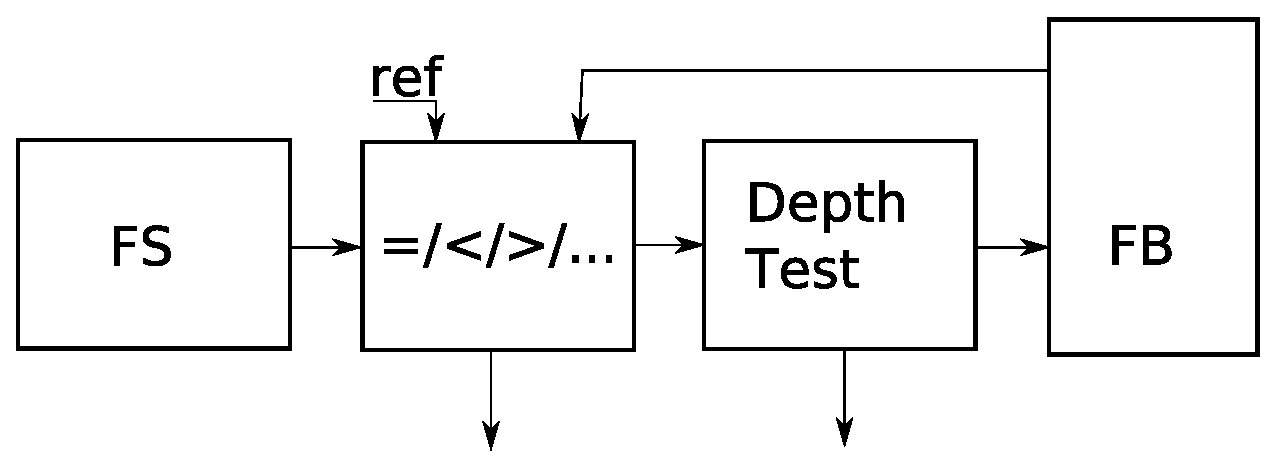
\includegraphics[width=\textwidth]{pics/shadows/shadowVolumes/stencil-test.eps}

  \vfill

  \begin{minted}[frame=lines]{c++}
    glEnable(GL_STENCIL_TEST);

    glStencilFuncSeparate(face, func, ref, mask);
  \end{minted}

  \vfill
  \begin{itemize}
    \item func $\in$ \{GL\_ALWAYS, GL\_NEVER, GL\_LESS, GL\_GREATER, ...\}
    \item if(S\&mask == ref\&mask)//GL\_EQUAL
  \end{itemize}
\end{frame}

\begin{frame}
  \frametitle{Změny stencil bufferu}

  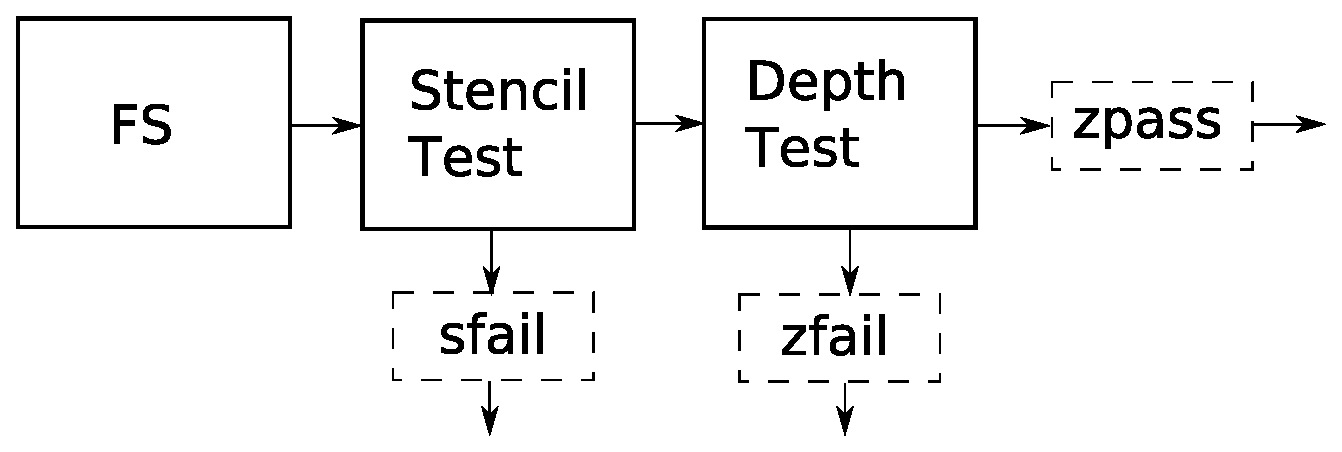
\includegraphics[width=\textwidth]{pics/shadows/shadowVolumes/stencil-test2.eps}

  \vfill

  glStencilOpSeparate(face, sfail, zfail, zpass);

  \begin{itemize}
    \item GL\_KEEP, GL\_ZERO, GL\_REPLACE, GL\_INVERT
    \item GL\_INCR, GL\_DECR, GL\_INCR\_WRAP, GL\_DECR\_WRAP
  \end{itemize}

  \vfill

  $255 + 1 = 255 \Longleftrightarrow $ GL\_INCR

  $255 + 1 = 0 \Longleftrightarrow $ GL\_INCR\_WRAP

\end{frame}




\begin{frame}
  \frametitle{Shadow Volumes}
  \begin{itemize}
    \item Shadow volume je metoda pro tvorbu přesných tvrdých stínů.
    \item Vyžaduje 3 kreslící průchody.
    \item První průchod - vykreslení scény pouze s ambientním světlem.
    \item Druhý průchod - vykreslení stínové geometrie a vytvoření stencilové masky.
    \item Třetí průchod - vykreslení scény s difuzním a spekulárním světlem s využitím stencilové masky.
    \item Existují dvě verze: zpass a zfail.
  \end{itemize}
\end{frame}

\begin{frame}
  \frametitle{Shadow Volumes algoritmus}
  \begin{enumerate}
    \item 1. kreslící průchod - ambietní světlo
      \begin{enumerate}
        \item Vykresli scénu s ambietním osvětlením.
      \end{enumerate}
    \item 2. kreslící průchod - tvorba stencilové masky
      \begin{enumerate}
        \item Vypni kreslení barvy a modifikaci depth bufferu.
        \item Nastav stencilovou operaci na incrementaci u přivrácených trojúhelníku a dekrementaci při odvrácených trojúhelníků.
        \item Povol zápis do stencil bufferu.
        \item Vykresli stínovou geometrii - vytvoří se stencilová maska.
        \item Vypni zápis do stencilového bufferu.
        \item Povol kreslení barvy a modifikaci depth bufferu.
      \end{enumerate}

    \item 3. kreslící průchod - difuzní, spekulární svetlo
      \begin{enumerate}
        \item Zapni stencil test -  při stencilové hodnotě 0 test projde.
        \item Vykresli scénu s difuzním a spekuláním osvětlením.
        \item Vypni stencil test.
      \end{enumerate}
  \end{enumerate}
\end{frame}

\begin{frame}
    \frametitle{Jak na stínová tělesa?}

    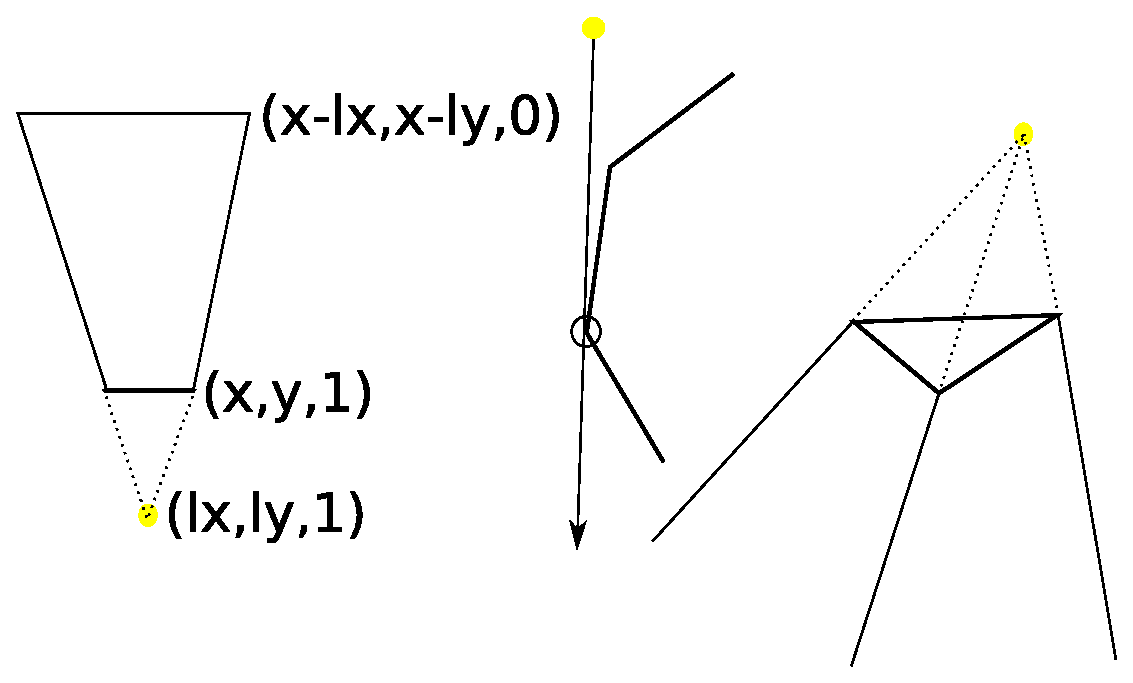
\includegraphics[width=\textwidth]{pics/shadows/shadowVolumes/shom.eps}

    \vfill

    \begin{itemize}
        \item Siluetu protáhnout do nekonečna
        \item Ideální bod $(x,y,z,0)$
    \end{itemize}
\end{frame}

\begin{frame}[fragile]
  \frametitle{Shadow volumes - tvorba geometrie}
  \begin{columns}[T]
    \begin{column}{.44\textwidth}
      {\tiny
        \begin{minted}[frame=lines]{glsl}
          #version 330
          layout(triangles)in;
          layout(triangle_strip,max_vertices=10)out;
          uniform mat4 MVP,M;//matice
          uniform vec4 LightPosition;//pozice svetla
          void main(){
            vec4 LP=M*LightPosition;
            vec4 p[6];
            p[0]=gl_in[0].gl_Position;//body trojuhelniku
            p[1]=gl_in[1].gl_Position;
            p[2]=gl_in[2].gl_Position;
            p[3]=vec4(gl_in[0].gl_Position.xyz*LP.w-LP.xyz,0);//v nekonecnu
            p[4]=vec4(gl_in[1].gl_Position.xyz*LP.w-LP.xyz,0);
            p[5]=vec4(gl_in[2].gl_Position.xyz*LP.w-LP.xyz,0);
            vec3 N=normalize(cross((p[1]-p[0]).xyz,(p[2]-p[0]).xyz));
            float Distance=dot(N,LP.xyz)-dot(N,p[0].xyz);
            if(Distance<=0){//otocime volume vnitrkem ven
              vec4 c=p[0];p[0]=p[1];p[1]=c;
              c=p[3];p[3]=p[4];p[4]=c;
            }
            gl_Position=MVP*p[0];EmitVertex();
            gl_Position=MVP*p[1];EmitVertex();
            gl_Position=MVP*p[3];EmitVertex();
            gl_Position=MVP*p[4];EmitVertex();
            gl_Position=MVP*p[5];EmitVertex();
            gl_Position=MVP*p[1];EmitVertex();
            gl_Position=MVP*p[2];EmitVertex();
            gl_Position=MVP*p[0];EmitVertex();
            gl_Position=MVP*p[5];EmitVertex();
            gl_Position=MVP*p[3];EmitVertex();
            EndPrimitive();
          }
        \end{minted}
      }
    \end{column}
    \begin{column}{.48\textwidth}
      \begin{figure}[h]
        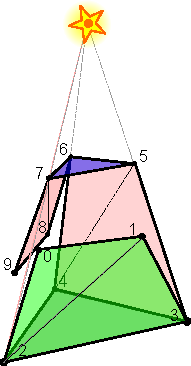
\includegraphics[width=3cm,keepaspectratio]{pics/shadows/shadowVolumes/perTriangle.pdf}
      \end{figure}
    \end{column}
  \end{columns}

\end{frame}

\begin{frame}
  \frametitle{Shadow Volumes ZPass}
  \begin{figure}[h]
    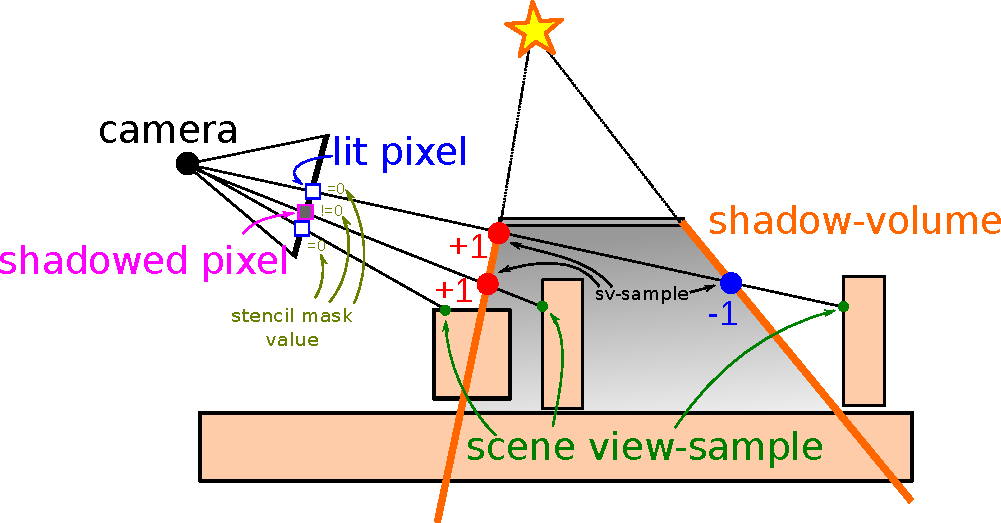
\includegraphics[width=11.5cm,keepaspectratio]{pics/shadows/shadowVolumes/ZPass}
  \end{figure}
\end{frame}

\begin{frame}[fragile]
  \frametitle{Shadow Volumes - 1. průchod}

  \begin{minted}[frame=lines]{c++}
//activate phong program
glUseProgram(phongProgram);

//enable ambient lighting
glProgramUniform4fv(phongProgram,
  lightAmbientColorUniform,light.amientColor);

//disable diffuse and specular lighting
glProgramUniform4f (phongProgram,
  lightDiffuseColorUniform,0,0,0,0);
glProgramUniform4f (phongProgram,
  lightSpecularColorUniform,0,0,0,0);

//draw the scene
glMultiDrawElementsIndirect(...);
  \end{minted}
\end{frame}

\begin{frame}[fragile]
  \frametitle{Shadow Volumes - 2. průchod}

  \begin{minted}[frame=lines]{c++}
//activate shadow volume geometry program
glUseProgram(shadowVolumeProgram);

glColorMask(GL_FALSE,GL_FALSE,GL_FALSE,GL_FALSE);
glDepthMask(GL_FALSE);

glEnable(GL_STENCIL_TEST);
glStencilFunc(GL_ALWAYS,0,0);
glStencilOpSeparate(GL_FRONT,GL_KEEP,GL_KEEP,GL_INCR_WRAP);
glStencilOpSeparate(GL_BACK ,GL_KEEP,GL_KEEP,GL_DECR_WRAP);

//draw the shadow geometry
glMultiDrawElementsIndirect(...);

glStencilOp(GL_KEEP,GL_KEEP,GL_KEEP);
glDepthMask(GL_TRUE);
glColorMask(GL_TRUE,GL_TRUE,GL_TRUE,GL_TRUE);
  \end{minted}
\end{frame}

\begin{frame}[fragile]
  \frametitle{Shadow Volumes - 3. průchod}

  \begin{minted}[frame=lines]{c++}
//activate phong program
glUseProgram(shadowVolumeProgram);

glProgramUniform4f (phongProgram,
  lightAmbientColorUniform,0,0,0,0);
glProgramUniform4f (phongProgram,
  lightDiffuseColorUniform,light.diffuseColor);
glProgramUniform4f (phongProgram,
  lightSpecularColorUniform,light.specularColor);

glStencilFunc(GL_EQUAL,0,0xff);

//draw the scene
glMultiDrawElementsIndirect(...);

glDisable(GL_STENCIL_TEST);
  \end{minted}
\end{frame}


\begin{frame}
    \frametitle{Víc světel}
    $N$ světel znamená $2^N$ kombinací zastíněností :( Co s tím?
    \pause\vfill
    \begin{equation*}
        \begin{array}{lcll}
            L &=& k_e + \sum\limits_{i=1}^n k_a \cdot L_{a(i)}   & + k_d \cdot L_{d(i)} \cdot (\vec L_i \cdot \vec N) + k_s \cdot L_{s(i)} \cdot (\vec V \cdot \vec{R_i})^n \\
            L_0 &=& k_e + \sum\limits_{i=1}^n k_a \cdot L_{a(i)} & \\
            L_i &=& L_{i-1}                                      & + k_d \cdot L_{d(i)} \cdot (\vec L_i \cdot \vec N) + k_s \cdot L_{s(i)} \cdot (\vec V \cdot \vec{R_i})^n
        \end{array}
    \end{equation*}
    \pause\vfill
    \begin{itemize}
        \item Vykreslit scénu s ambient+emission
        \item Pro každé světlo
        \begin{itemize}
            \item Připravit stencil buffer
            \item Přiblendovat diffuse+specular
            \item (glDepthFunc(GL\_LEQUAL), glBlendFunc(GL\_ONE, GL\_ONE))
        \end{itemize}
    \end{itemize}
\end{frame}

\begin{frame}
    \frametitle{Výhody a nevýhody}
    
    $+$
    \begin{itemize}
        \item Dynamické scény
        \item Problematické scény
        \item Sedí na pixel přesně
    \end{itemize}

    \vfill
    $-$
    \begin{itemize}
        \item Pomalé
        \item Závislé na fillrate
        \item Konstrukce stínových těles
        \item Jen ostré stíny
    \end{itemize}
\end{frame}

\begin{frame}
    \frametitle{Problém...}
    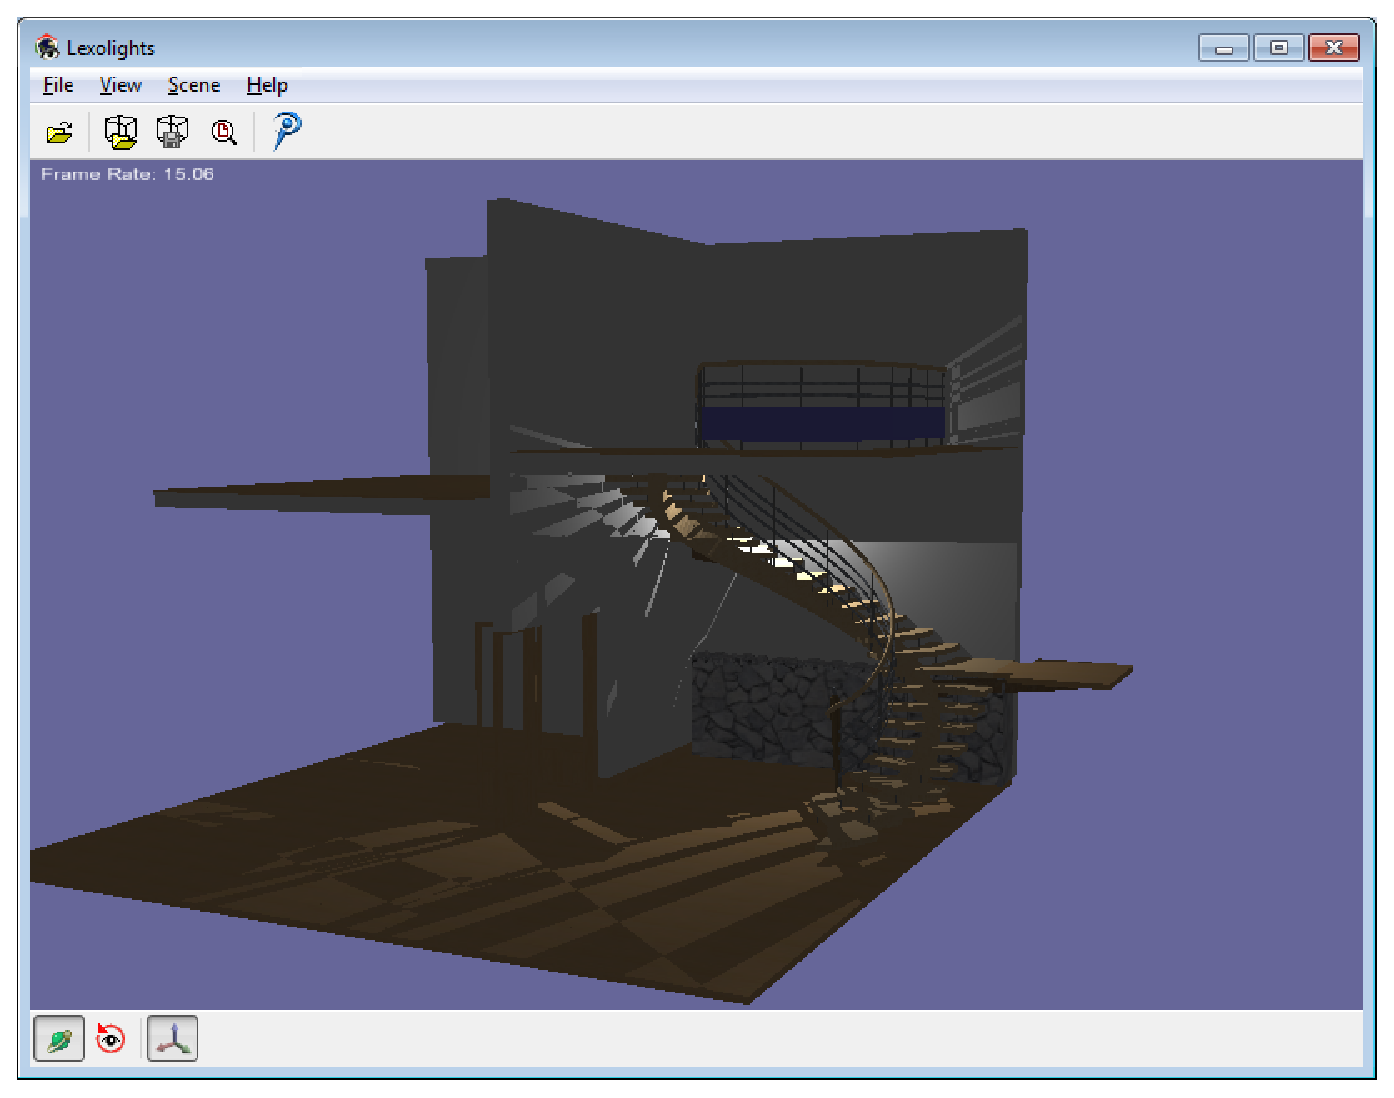
\includegraphics[width=3in]{pics/shadows/shadowVolumes/ZPass-fail.eps}
    \pause\vfill
    Stačí vlézt dovnitř stínového tělesa.
\end{frame}

\begin{frame}
    \frametitle{Z\_PASS vs. Z\_FAIL}
    Pixel je ve stínu když paprsek vletí {\color{red}dovnitř} a nevyletí {\color{blue}ven}.
    \begin{columns}[c]
    \column{.5\textwidth}
        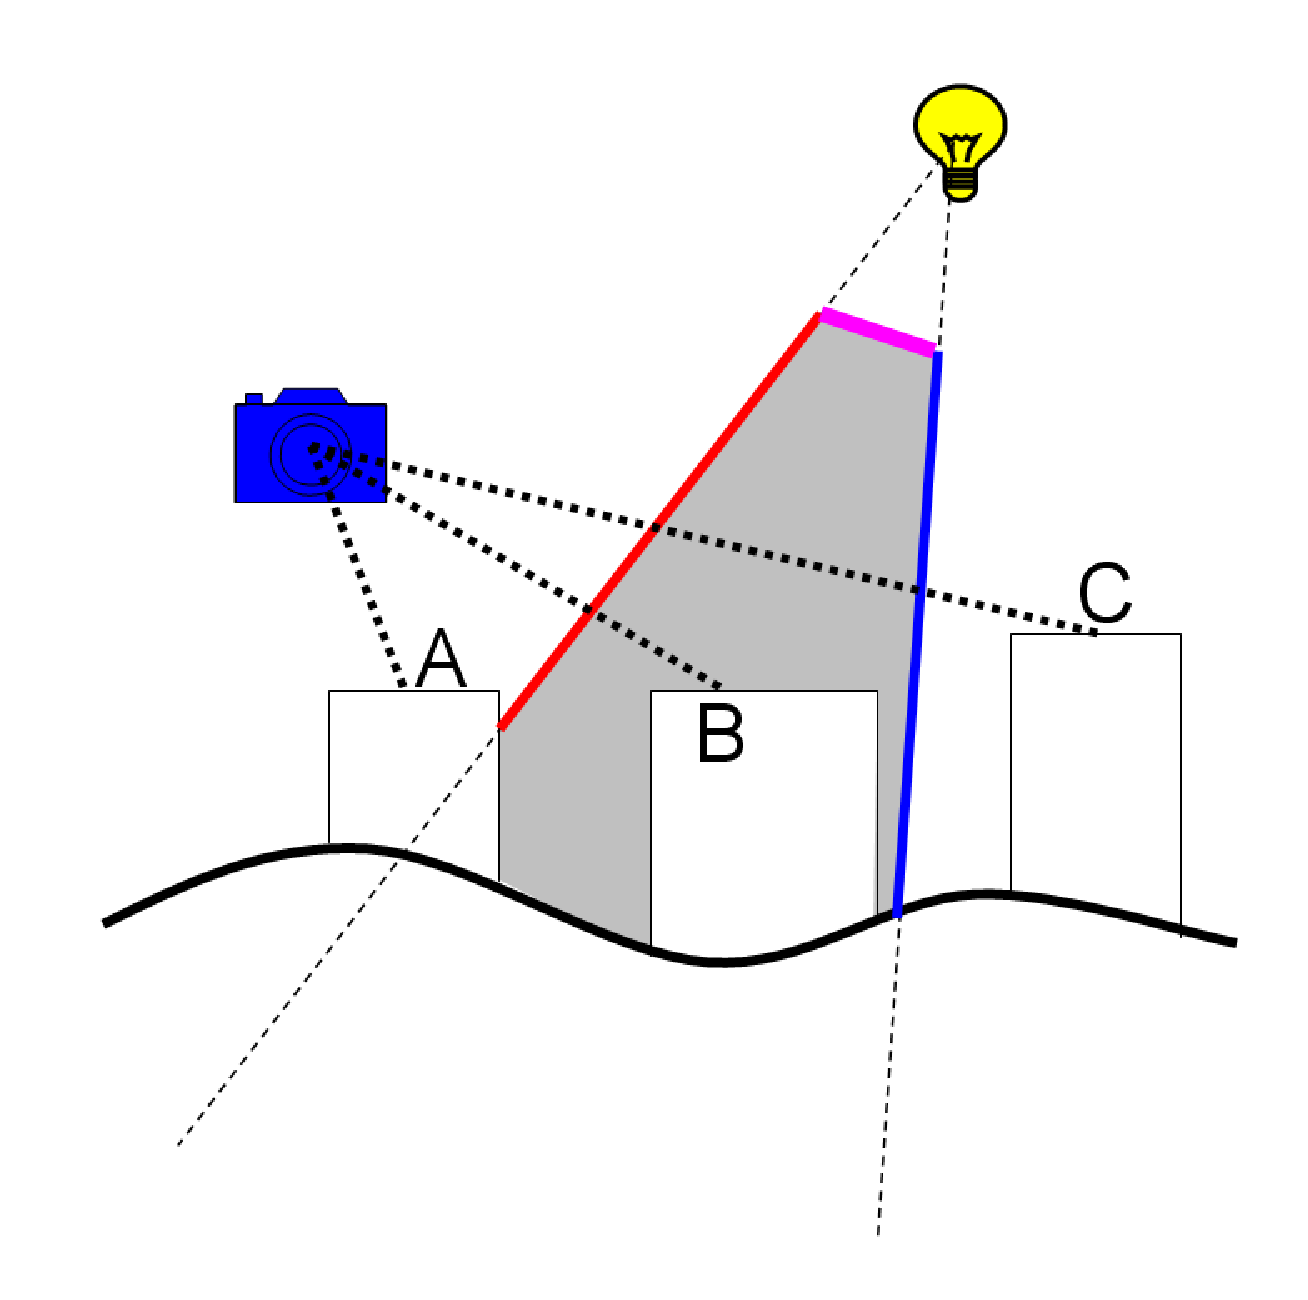
\includegraphics[width=\textwidth]{pics/shadows/shadowVolumes/ShadowVolume.eps}
    \column{.5\textwidth}
        Z\_PASS : \\
        Počítám viditelné pixely \\
        {\color{red} +1}, {\color{blue} -1}
        \vfill
        Z\_FAIL : \\
        Počítám neviditelné pixely
        {\color{red} -1}, {\color{blue} +1}
    \end{columns}
    \pause\vfill
    glStencilOpSeparate(GL\_FRONT, GL\_KEEP, GL\_DECR\_WRAP, GL\_KEEP);\\
    glStencilOpSeparate(GL\_BACK, GL\_KEEP, GL\_INCR\_WRAP, GL\_KEEP);    
\end{frame}

\begin{frame}
    \frametitle{Další zádrhel}
    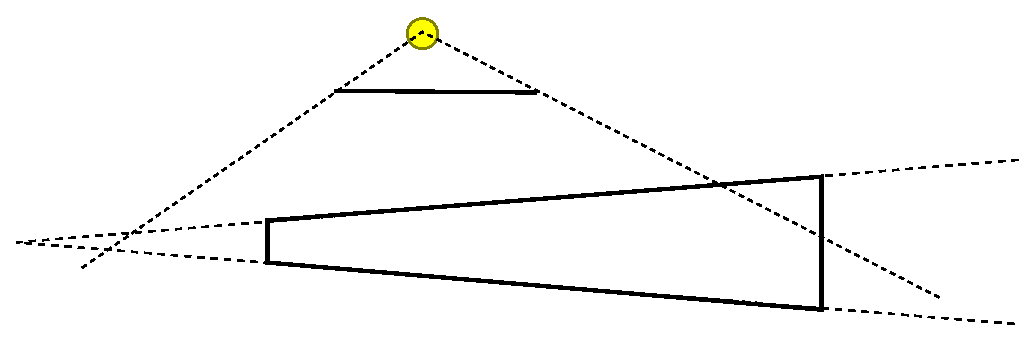
\includegraphics[width=\textwidth]{pics/shadows/shadowVolumes/svol-cap.eps}
    \begin{itemize}
        \item Stínové těleso musí být uzavřené.
        \item A jeho stěny musí být "viditelné".
        \item Problém je far-plane.
    \end{itemize}
\end{frame}

\begin{frame}
  \frametitle{Shadow Volumes ZFail}
  \begin{figure}[h]
    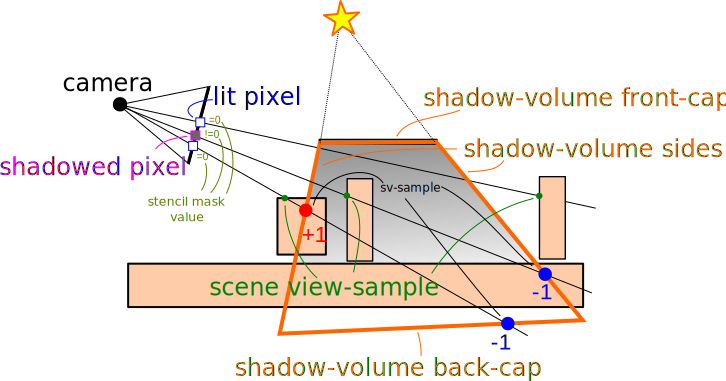
\includegraphics[width=11.5cm,keepaspectratio]{pics/shadows/shadowVolumes/ZFail}
  \end{figure}
\end{frame}

\begin{frame}[fragile]
  \frametitle{Shadow Volumes - 2. průchod modifikace}

  \begin{minted}[frame=lines]{c++}
//activate shadow volume geometry program
glUseProgram(shadowVolumeProgram);
glProgramUniformMatrix4fv(shadowVolumeProgram,mvpUniform,
  1,GL_FALSE,infiniteProjectionMatrix);

glColorMask(GL_FALSE,GL_FALSE,GL_FALSE,GL_FALSE);
glDepthMask(GL_FALSE);

glEnable(GL_STENCIL_TEST);
glStencilFunc(GL_ALWAYS,0,0);
glDepthFunc(GL_LESS);
glStencilOpSeparate(GL_FRONT,GL_KEEP,GL_INCR_WRAP,GL_KEEP);
glStencilOpSeparate(GL_BACK ,GL_KEEP,GL_DECR_WRAP,GL_KEEP);

//draw the shadow geometry with caps
glMultiDrawElementsIndirect(...);

glStencilOp(GL_KEEP,GL_KEEP,GL_KEEP);
glDepthMask(GL_TRUE);
glColorMask(GL_TRUE,GL_TRUE,GL_TRUE,GL_TRUE);
  \end{minted}
\end{frame}


\begin{frame}
    \frametitle{Nekonečná projekce}
    \begin{align*}
        \lim_{\mathrm{far} \to +\infty}\begin{pmatrix}
            \frac{2\mathrm{near}}{\mathrm{right}-\mathrm{left}}&0&\frac{\mathrm{right}+\mathrm{left}}{\mathrm{right}-\mathrm{left}}&0\\
            0&\frac{2\mathrm{near}}{\mathrm{top}-\mathrm{bottom}}&\frac{\mathrm{top}+\mathrm{bottom}}{\mathrm{top}-\mathrm{bottom}}&0\\
            0&0&-\frac{\mathrm{far}+\mathrm{near}}{\mathrm{far}-\mathrm{near}}&-\frac{2\mathrm{near}\mathrm{far}}{\mathrm{far}-\mathrm{near}}\\
            0&0&-1&0
        \end{pmatrix} \\
        = \begin{pmatrix}
            \frac{2\mathrm{near}}{\mathrm{right}-\mathrm{left}}&0&\frac{\mathrm{right}+\mathrm{left}}{\mathrm{right}-\mathrm{left}}&0\\
            0&\frac{2\mathrm{near}}{\mathrm{top}-\mathrm{bottom}}&\frac{\mathrm{top}+\mathrm{bottom}}{\mathrm{top}-\mathrm{bottom}}&0\\
            0&0&-1&-2\mathrm{near}\\
            0&0&-1&0
        \end{pmatrix}
    \end{align*}
    \pause\vfill
    \begin{itemize}
        \item[:)] Vidíme do nekonečna.
        \item[?] Co z-test? Dělíme nekonečnou délku na konečný počet dílků.
    \end{itemize}
\end{frame}

\begin{frame}
    \frametitle{Z-buffer a nekonečno}
    \begin{align*}
        P(z) &= \frac{z - 2n}{z} = 1 - \frac{2n}{z} & \text{ Dopředu je $-z$}
    \end{align*}
    \pause\vfill
    \begin{align*}
        P(n) &= -1 & P(\infty) &=  1 \\
        P(2n) &= 0 & P(4n) &= 1/2
    \end{align*}
    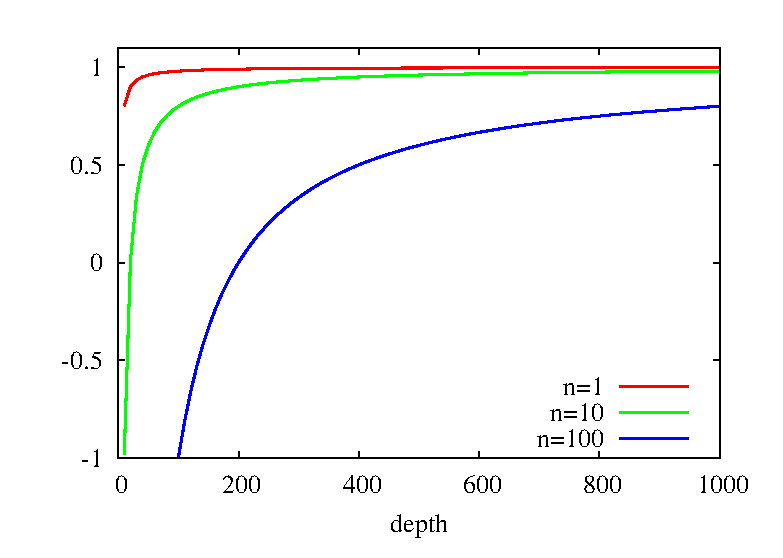
\includegraphics[width=.5\textwidth]{pics/shadows/shadowVolumes/plot/infdepth.eps}
    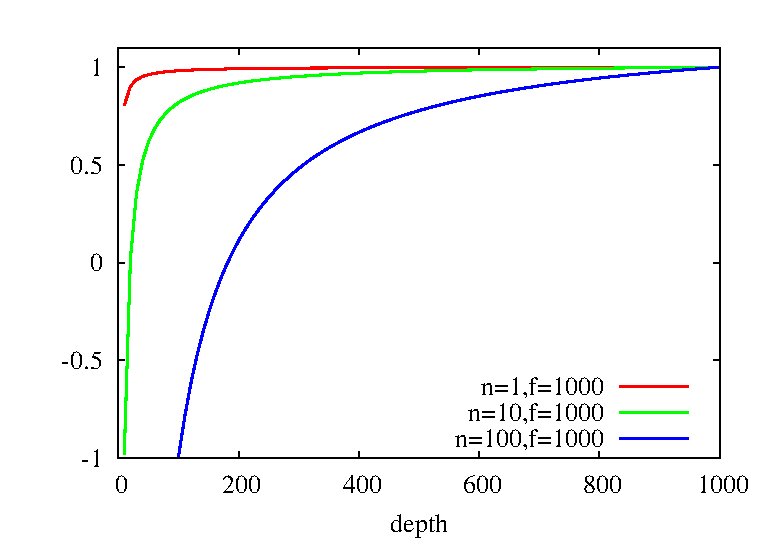
\includegraphics[width=.5\textwidth]{pics/shadows/shadowVolumes/plot/findepth.eps}
    \begin{itemize}
        \item[:)] Většina hodnot z-bufferu je v "rozumné" vzdálenosti.
    \end{itemize}
\end{frame}

